\chapter{Molecular Structure}
\label{cha:molecular-structure}
\index{molecular structure}
We are to deal with the structure and energetics of molecules in a
very heuristic fashion, deriving the energies and importance 
of various transitions.   

The simplest molecules are the diatomic molecules such as H$_2$, CO,
{\em etc.}. They are also among the most abundant in the universe, so
we are going to restrict our attention to these two-atom molecules.

\section{The Born-Oppenheimer Approximation}
\label{sec:born-oppenh-appr}
\index{molecular structure!Born-Oppenheimer approximation}
\index{Born-Oppenheimer approximation}

The problem of understanding the structure of molecules initially
appears formidable.  At a basic level the equations are no longer
spherically symmetric.  This is a real difficulty.  For diatomic
molecules there is still a rotational symmetry about the line
connecting the two nuclei.  The key simplification is that the
electrons whip around a lot faster than the nuclei, so one can
approximate the sitution by assuming that the electrons sit in a
particular eigenstate of the potential with the two ions fixed.
The ions on the other hand experience an effective potential as a
function of their separation that includes the effects of the
electrons (whose state we have already calculated).  This in the {\em
  Born-Oppenheimer} approximation.

By looking a moleculle in terms of the electrons and the nuclei
separately, we can estimate the energies of the various transitions of
the molecule.  Let's assume that the ions are separated by a distance
$a \sim a_0$.  By the uncertainty principle the momentum of the
electrons will be on the order of $\hbar / a$, and the typical energy
of electronic transitions will be
\begin{equation}
E_\textrm{\scriptsize elec} \sim \frac{p^2}{m} \sim 
\frac{\hbar^2}{m a^2} \sim \alpha^2 m c^2 \sim 1~\textrm{eV}
\label{eq:10000}
\end{equation}
or the visibile, near-infrared and ultraviolet.

The nuclei are separated by a distance of order $a$ as well and the
typical energy change from moving nuclei over a distance $a$ is the
electronic energy (Eq.~\ref{eq:10000}), so we can define a spring
constant for the nuclei
\begin{equation}
  k \sim \frac{E_\textrm{\scriptsize elec}}{a^2} \sim \frac{\hbar^2}{m a^4}
\label{eq:10001}
\end{equation}
yielding a vibrational energy corresponding to changes in the distance
between the nuclei of 
\begin{equation}
E_\textrm{\scriptsize vib} \sim \hbar \omega = \hbar \left
  (\frac{k}{M} \right )^{1/2}
= \hbar \left ( \frac{\hbar^2}{m M a^4} \right )^{1/2}
= \left ( \frac{m}{M} \right )^{1/2} \frac{\hbar^2}{m a^2}
\sim 0.01-0.1~\textrm{eV}.
\label{eq:10002}
\end{equation}
These energies fall in the infrared.  Finally the molecule can change
its rotational state.  The angular momentum of the molecule is
quanized in units of $\hbar$ so we would expect transitions with
energies of the order of 
\begin{equation}
E_\textrm{\scriptsize rot} \sim \frac{\hbar^2 L \left (L+1\right) }{2
  I} = \frac{\hbar^2 L \left (L+1\right )}{M
  a^2} = \frac{m}{M} \frac{\hbar^2}{m a^2} L \left (L+1\right )\sim 10^{-3}~\textrm{eV}.
\label{eq:10003}
\end{equation}
Because the typical energies of the various transitions are well
separated we can to a good approximate consider each of them
separately, justifying the Born-Oppenheimer approximation.

\section{The H$_2^+$ Molecular Ion}

An example which illustrates much of the physics of diatomic molecules
is the hydrogen molecular ion H$_2^+$.  The Schrodinger equation for
this system is
\begin{equation}
\left [ -\frac{\hbar^2}{2 \mu_{AB}} \nabla^2_{\bf R}
  -\frac{\hbar^2}{2 \mu_e} \nabla^2_{\bf r} - \frac{e^2}{r_A} -
\frac{e^2}{r_B} + \frac{e^2}{R} - E \right ] \psi({\bf r},{\bf R}) = 0  
\label{eq:573}
\end{equation}
$\mu_{AB}$ is the reduced mass of the two protons, $M/2$ and $\mu_e$
is the reduced mass of the electron relative to the two protons
$\approx m_e$.   $r_A$ and $r_B$ are the distances between the
electron and the two protons and $R$ is the distance between the two
protons.    The key to the Born-Oppenheimer approximation is first to
hold ${\bf R}$ fixed and neglect the first kinetic energy term and
solve for the electronic wavefunction $\chi_j({\bf r};{\bf R})$.
\begin{equation}
\left [ 
  -\frac{\hbar^2}{2 \mu_e} \nabla^2_{\bf r} - \frac{e^2}{r_A} -
\frac{e^2}{r_B} + \frac{e^2}{R} - E_j({\bf R}) \right ] \chi_j({\bf r};{\bf R}) = 0  
\label{eq:574}
\end{equation}
where the semicolon in the $\chi_j$ function encourages us to think of
${\bf R}$ as a parameter.  We try various values of ${\bf R}$ and
solve for $\chi_j({\bf r};{\bf R})$ each time. The solutions to this
equation are called {\em molecular orbitals}.

After the electronic wavefuntion is calculated as a function of $R$,
we can determine the proton wavefunction.  The proton wavefunction
satisfies the one-body Schrodinger equation 
\begin{equation} 
\left [
-\frac{\hbar^2}{2 \mu_{AB}} \nabla^2_{\bf R} + E_j({\bf R}) - E \right
] F_j({\bf R}) = 0 
\label{eq:575}
\end{equation}

Eq.~\ref{eq:574} is generally to difficult to solve directly, so one generally
picks a trial wavefunction and calculates the value of the energy for
this function.  One can prove that the ground state eigenvalue $E$ of the
Hamiltonian $H$
\begin{equation}
E \leq  \langle \psi | H | \psi \rangle
\label{eq:576}
\end{equation}
where $\psi$ is any normalized wavefunction.  This is the basis of the
{\em Rayleigh-Ritz variational method}.

For the case in point, we will guess that the wavefunction of the
electron is a {\bf l}inear {\bf c}ombination of {\bf a}tomic {\bf
  o}rbitals (LCAO), specifically the $1s$ state of hydrogen.
\begin{equation}
\chi_g = \frac{1}{\sqrt{2}} \left ( \psi_{1s} (r_A) + \psi_{1s}(r_B)
  \right )
\label{eq:577}
\end{equation}
and 
\begin{equation}
\chi_u = \frac{1}{\sqrt{2}} \left ( \psi_{1s} (r_A) - \psi_{1s}(r_B)
  \right )
\label{eq:578}
\end{equation}
The $g$ and the $u$ refer to {\em gerade} (even-parity) and {\em
  ungerade} (odd-parity) wavefunctions.

We can substitute these trial wavefunctions into the Hamiltonian in
Eq.~(\ref{eq:574}) to find an upper limit on the value of $E_j({\bf R})$.  We
obtain
\begin{equation}
E_{gu} (R) = E_{1s} + \frac{e^2}{R} \frac{(1 +
  R/a_0)e^{-2R/a_0}\pm[1-(2/3)(R/a_0)^2] e^{-R/a_0}}{1\pm[1+R/a_0+(R/a_0)^2/3]e^{-R/a_0}}
\label{eq:579}
\end{equation}
where the upper (positive) sign corresponds to the {\em gerade} configuration.
Fig.~\ref{fig:h2p} depicts the energy of the electronic configuration
and Fig.~\ref{fig:psiug} shows the electron density for the two
orbitals.  We see that the only the gerade state binds in the case.
From the picture of the electron probability density we can see why
this is the case.  In the gerade case, the electron lies in between
the two ions so it can shield the charge of one ion from the other.
In the ungerade state because it has odd parity, the electron cannot
lie on the midplane between the ions so the shielding is much less 
effective.  
{
\begin{figure}
\begin{center}
\begin{tikzpicture}
\begin{scope}[yscale=20,smooth]
\clip (0,-0.1) rectangle (6,0.2);
\draw[color=red] plot file{xegx.dat} ;
\draw[color=blue] plot file{xeux.dat} ;
\draw[dashed] plot file{xmorsex.dat} ;
\end{scope}
\begin{scope}[yscale=20]
\draw[->] (-0.2,-0.1) -- (6.2,-0.1) node[right] {$\frac{R}{a_0}$}; 
\draw[->] (0,-0.12) -- (0,0.22) node[above] {$\frac{E a_0}{e^2}$};
\foreach \x in {1,...,6} 
  \draw (\x,-0.1) node [below] {$\x$};
\foreach \x in {-0.1,0,0.1,0.2}
  \draw (-0.1,\x) node [left] {$\x$};
\end{scope}
\end{tikzpicture}
\end{center}
%\centering
%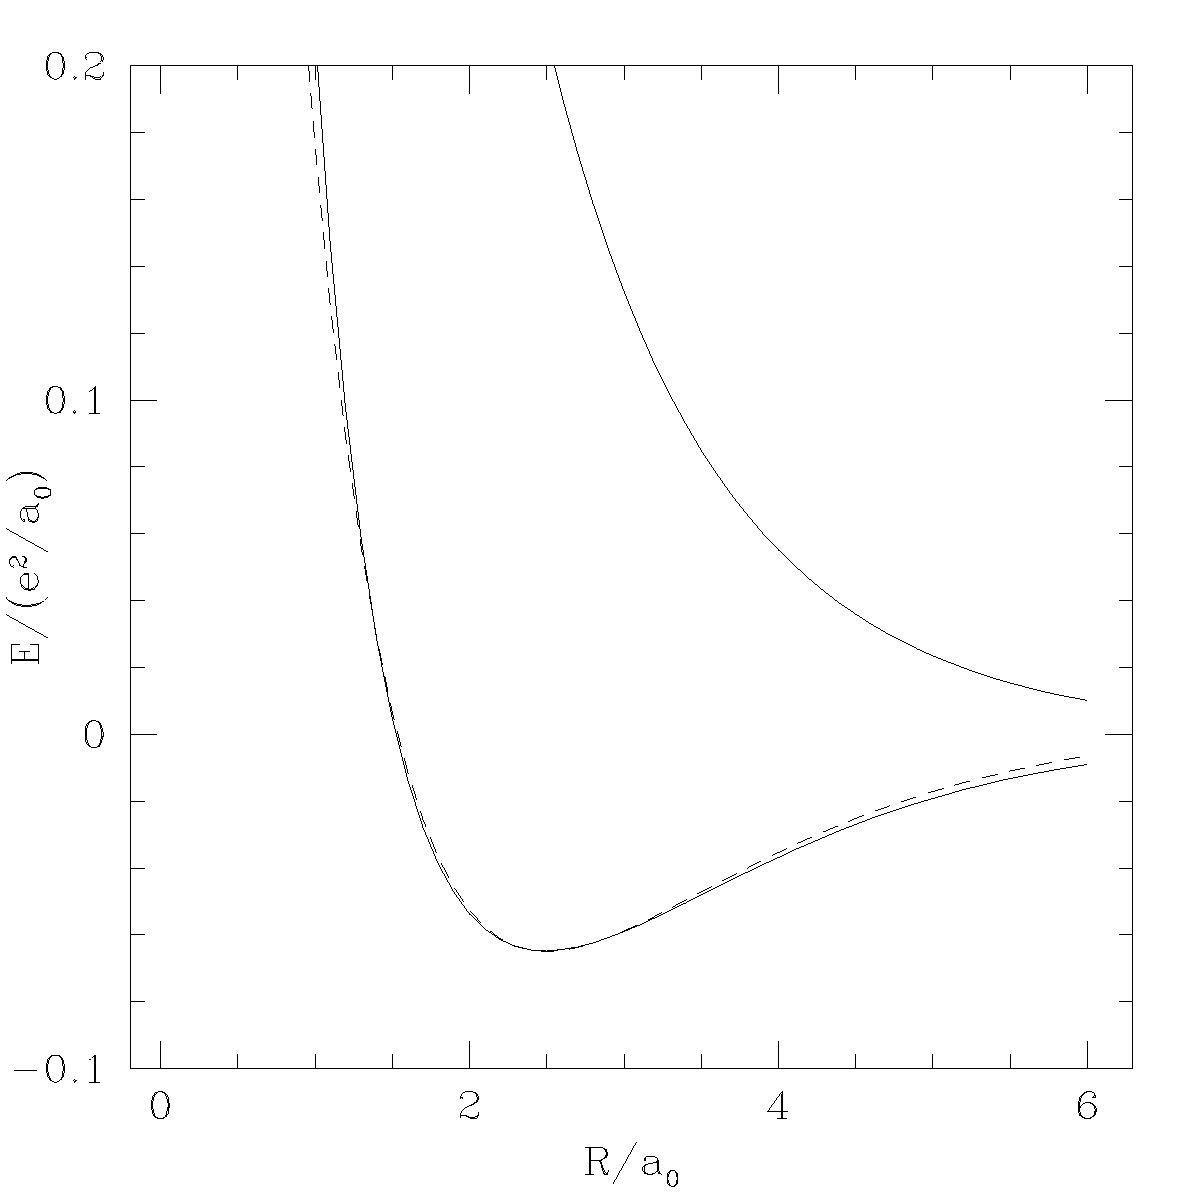
\includegraphics[width=0.45\textwidth]{h2p} 
\caption{$E_{u}$ (upper curve) and $E_g$ (lower curve) for
  H$_2^+$. The dashed curve is a well-fit Morse potential for $E_g(R)$.}
\label{fig:h2p}
\end{figure}
}
{
\begin{figure}
\centering
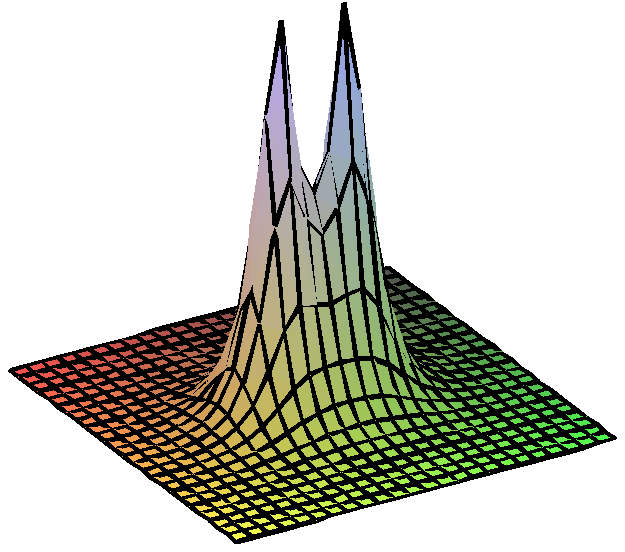
\includegraphics[width=0.45\textwidth]{psig} 
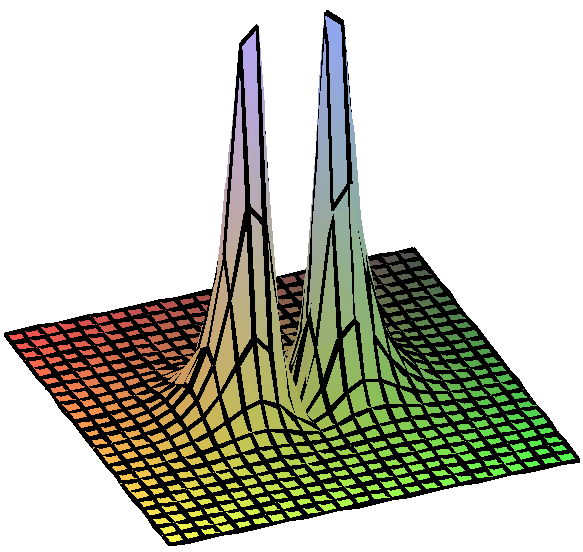
\includegraphics[width=0.45\textwidth]{psiu} 
\caption{$|\psi_g|^2$ (left) and $|\psi_u|^2$ (right) for H$_2^+$ with
  $R=2 a_0$.}
\label{fig:psiug}
\end{figure}
}

For molecules with more than one electron, we find that the Hund's rule
for the total spin of a system is reversed for molecules.  The states
with even parity (gerade) tend to bond.  Because the spatial wavefunction is
even with respect interchanging the electrons their spins must be
antiparallel. 

\section{Molecular Excitations}
\label{sec:molec-excit}
\index{molecular structure!excitations}

The energy states of molecule may be excited in three ways: {\em
  electronic}, {\em vibrational}, and {\em rotational}.  Let's start
  with the least energetic of these.

We can get a first-order understanding of the rotational states of a
molecule simply looking at the Schrodinger equation for the ions
\be 
\left [
-\frac{\hbar^2}{2 \mu_{AB}} \left ( \frac{d^2}{dR^2} -
\frac{L(L+1)}{R^2} \right )  + E_j({\bf R}) - E \right
] F_j({\bf R}) = 0 
\label{sec:molec-excit-1}\end{equation}
where we have solved the angular wavefunction in terms of spherical
harmonics like we did for hydrogen.  In Fig.~\ref{fig:h2p} we saw that
the function $E_j({\bf R})$ varies over atomic distances $\sim a_0$.
On the other hand because the mass of the ions is much larger than
that of the electrons we expect the wavefunction of the ions to be
localized in a region $\sim a_0 m/M \ll a_0$.  Over this small region
we can expand the function $E_j(R)$ about its minimum $R_0$
\begin{equation}
E_j(R) = E_j(R_0) + (R-R_0) \left [ \dd{E_j(R)}{R} \right ]_{R=R_0} +
\frac{1}{2} (R-R_0)^2 \left [ \frac{d^2 E_j(R)}{d R^2} \right
]_{R=R_0} + \cdots
\label{eq:580}
\end{equation}
where the second term vanishes because $R_0$ is the minimum so we have
\be 
\left [
-\frac{\hbar^2}{2 \mu_{AB}} \frac{d^2}{dR^2} -
\frac{\hbar^2}{2\mu_{AB}} \frac{L(L+1)}{R^2} + E_j(R_0) + \frac{1}{2}
k (R-R_0)^2 - E \right
] F_j({\bf R}) = 0 
\label{sec:molec-excit-2}\end{equation}
so we have
\begin{equation}
E = E_j(R_0) + \hbar \omega_0 \left ( v + \frac{1}{2} \right ) + \frac{\hbar^2}{2\mu_{AB}} \frac{L(L+1)}{R_0^2}
\label{eq:581}
\end{equation}
where $\omega_0 = (k/\mu_{AB})^{1/2}$ and 
we have treated the rotational motion of the molecule
perturbatively.  We have effectively ignored the possible centrifugal
stretching of the molecule.  If we were to include the stretching of
the molecule we would have
\begin{equation}
E_\rmscr{rot} = \frac{\hbar^2}{2\mu_{AB}} \frac{L(L+1)}{R_0^2} \left [
  1 - \frac{2\hbar^2 L(L+1)}{k \mu_{AB} R_0^4} \right ]
\label{eq:582}
\end{equation}

We can get dipole transitions between the different rotational states
if
\begin{equation}
|d| = Z_1 e r_1 + Z_2 e r_2 + |d_e| \neq 0 
\label{eq:583}
\end{equation}
and $\Delta L = \pm 1$.  We see that homonuclear diatomic molecules
cannot emit dipole radiation due to changes in their rotational state.
The energy of the radiation is given by
\begin{equation}
E_{L+1,L} = \frac{\hbar^2 (L+1)}{\mu_{AB} R_0^2} \left [ 1 - 4
    \frac{\hbar^2 (L+1)^2}{k \mu_{AB} R_0^4} \right ]
\label{eq:584}
\end{equation}
This energy is $\sim e^2/a_0 (m/\mu_{AB})$ or $\sim 10^{-3}$~eV.

The transitions between vibrational states has a typical energy of 
$\sim e^2/a_0 (m/\mu_{AB})^{1/2}$ or $\sim 10^{-1}$~eV.  If one
includes the centrifugal effects one finds that 
\begin{equation}
E_v = \hbar \omega_L \left ( v + \frac{1}{2} \right )
\label{eq:585}
\end{equation}
where
\index{Morse function}
\index{molecular structure!Morse function}
\begin{equation}
\omega_L \approx \mu_{AB}^{-1/2} \left [ k + \frac{3 \hbar^2
    L(L+1)}{\mu_{AB} R_0^4} \right ]^{1/2}
\label{eq:586}
\end{equation}
Morse found that the internuclear potential can often be well
approximated by a function of the form
\begin{equation}
E_n(R) = E_{n,0} + B_n \left \{ 1 - \exp \left[ \beta_n \left ( R -
  R_0 \right )\right ] \right \}^2
\label{eq:587}
\end{equation}
The energy eigenvalues of this potential are
\begin{equation}
E_{nv} = \hbar \omega_{n0} \left ( v + \frac{1}{2} \right ) -
\frac{\hbar^2 \omega_0^2}{4 B_n} \left ( v + \frac{1}{2} \right )^2.
\label{eq:588}
\end{equation}
The vibrational levels get closer together as $v$ increases and there
are a finite number of vibrational levels
\begin{equation}
0 \leq v \leq \frac{(2\mu_{AB} B_n)^{1/2}}{\beta_n \hbar} - \frac{1}{2}
\label{eq:589}
\end{equation}

The selection rules for vibrational transtions are again $|d|\neq 0$ but
also $d|d|/dR \neq 0$.  We can change the vibrational level by $\Delta
v=\pm 1$ and we must also have $\Delta L=L_\textrm{\scriptsize lower}-L_\textrm{\scriptsize upper}=+1$ ($P$ branch) or $\Delta
L=-1$ ($R$ branch) or if there is an component of electronic orbital
or spin angular momentum along the internuclear axis $\Delta L=0$ ($Q$ branch).

Fig.~\ref{fig:molecule_trans} shows the three branches for
roto-vibrational transitions, if we neglect the stretching of the
molecule.    We see that
for the $R$ branch the transition energy decreases with increasing $L$.
For the $Q$ branch it is constant, and for the $P$ branch the
transition energy increases with increase $L$.  The centrifugal stretching reduces the spacing of the
angular momentum energy levels for large values of $L$ (Eq.~\ref{eq:584}), but it
stiffens the spring constant of the vibrational statres (Eq.~\ref{eq:586}).  The latter
dominates, so the stretching effect
tends to make the transition energies increase with increasing $L$ for
large values of $L$.  Fig.~\ref{fig:COCar} depicts the
roto-vibrational spectrum of CO (the most commonly observed molecule
in astrophysics --- it isn't the most common, what is the most common
molecule and why isn't it commonly observed?) from samples of car
exhaust.  The CO molecule does not exhibit a $Q$-branch which would
appear at about 2140~cm$^{-1}$.

The Fortrat diagram (Fig.~\ref{fig:fortrat})
depicts the transition energies for various roto-vibrational
transitions as a function of the rotational quantum number $L$.  The
figure shows the expected behaviour, especially for the ``22''
transitions for which all three branches are depicted.  For small
values of $L$ the $Q$-branch has constant energy with $L$ and then
begins to increase with increasing $L$  The energy of the $P$-branch
transitions decreases with increasing $L$, and the opposite occurs
for the $R$ branch.

\begin{figure}
\begin{center}
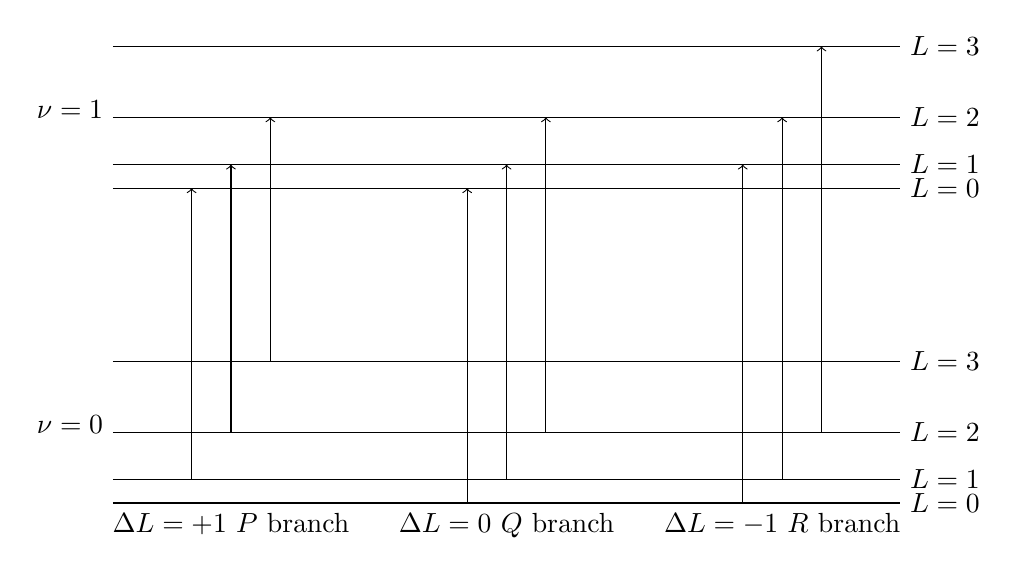
\begin{tikzpicture}
\foreach \nqn in {0,1}
  \foreach \lqn in {0,1,2,3} 
    \draw (0,\nqn*4+0.15*\lqn*\lqn+0.15*\lqn) -- (10,\nqn*4+0.15*\lqn*\lqn+0.15*\lqn) node [right] {$L=\lqn$};
\draw (0,5) node [left] {$\nu=1$} (0,1) node [left] {$\nu=0$};
\draw [->] (1,0.3) -- (1,4);
\draw [->] (1.5,0.9) -- (1.5,4.3);
\draw [->] (2,1.8) -- (2,4.9);
\draw (1.5,0) node [below] {$\Delta L=+1$ $P$ branch};
\draw [->] (4.5,0) -- (4.5,4);
\draw [->] (5,0.3) -- (5,4.3);
\draw [->] (5.5,0.9) -- (5.5,4.9);
\draw (5,0) node [below] {$\Delta L=0$ $Q$ branch};
\draw [->] (8,0) -- (8,4.3);
\draw [->] (8.5,0.3) -- (8.5,4.9);
\draw [->] (9,0.9) -- (9,5.8);
\draw (8.5,0) node [below] {$\Delta L=-1$ $R$ branch};
\end{tikzpicture}
\end{center}
\caption{Roto-Vibrational Transitions Neglecting Stretching}
\label{fig:molecule_trans}
\end{figure}

{\begin{figure}
\centering
\begin{tikzpicture}[scale=0.9]
\draw (0,0) node {
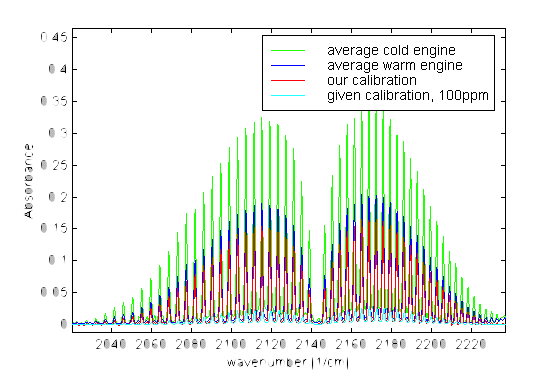
\includegraphics[width=0.9\textwidth,clip,trim=2.8cm 1.68cm 2.1cm 3.93cm]{CO_Car}
};
\draw [->] (-6.2,-3.25) -- (-6.2,3.05);
\draw [->] (-6.3,-3.15) -- (6.5,-3.15);
\draw (0,-3.6) node [below] {Wavenumber [cm$^{-1}$]};
\foreach \lam in {2040,2060,...,2220} 
   \draw (0.05893*\lam-125.5,-3.2) node [below] {\lam};
\foreach \abs in {0,0.1,0.2,0.3} 
   \draw (-6.2,18.6*\abs-3.15) node [left] {\abs};
\end{tikzpicture}
\caption{Absorption vs.\ Wavenumber for FTIR Spectroscopy of CO in car
  exhaust from {\tt
    http://home.swipnet.se/$\sim$w-74877/ftir/ftir.htm}.  Green is a
  cold engine, blue is a warm engine, red is a calibration reading and
cyan is a 100ppm calibration.}
\label{fig:COCar}
\end{figure}}
{\begin{figure}
\centering
\begin{tikzpicture}[scale=0.9]
\draw (0,0) node {
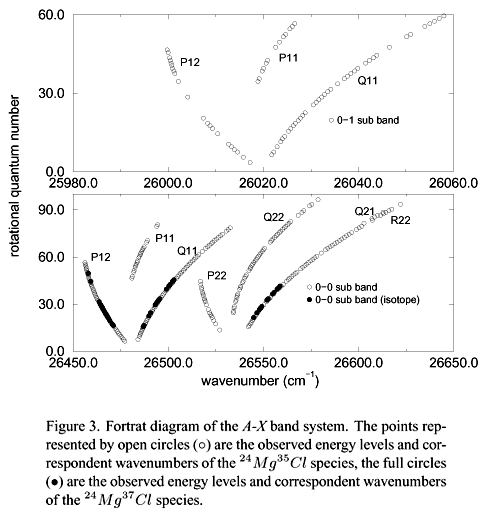
\includegraphics[width=0.9\textwidth,clip,trim=1cm 4.6cm 0 6.7cm]{fortrat.png} 
};
\draw (-6.5,0.3) node [rotate=90] {Rotational Quantum Number};
\end{tikzpicture}
\caption{A Fortrat diagram for $^{24}$Mg$^{35}$Cl and
  $^{24}$Mg$^{37}$Cl (isotope) from Gutterres et al. (2003),
  Braz. J. Phys. vol. 33}
\label{fig:fortrat}
\end{figure}}

In general each vibration transition includes a rotational transition
as well so one gets group of transitions.  The final wrinkle is that
electronic transitions in molecules whose energy $\sim 1$~eV
necessarily include changes in the rotational and vibrational state of
the molecule.  The general electronical-vibrational-rotational
spectrum takes the form of bands which can be resolved into individual
lines if the broadening is weak.

\section{Problems}
\begin{enumerate}

\item{\bf The Number of Levels}

I fit a Morse function to the potential of  H$_2^+$.  The parameters
were
\begin{equation}
E_{n,0} = -0.065 \frac{e^2}{a_0}, B_n = 0.07 \frac{e^2}{a_0}, \beta_n
= 0.7 a_0^{-1}, R_0 = 2.5 a_0
\label{eq:590}
\end{equation}
How many vibrational levels does H$_2^+$ have?   How many rotational
levels does each vibrational level typically have?

\item{\bf Nuclear Overlap}

Consider two deuterons bound by a single electron as in question (1).
What is the probability that the two deuterons lie on top of each
other, {\ie} that $R<4$~fermi, the diameter of the deuteron?   What is the
probability if the two deuterons are bound by a single muon, $m_\mu
\approx 207 m_e$?  You can find the eigenfunctions of the Morse
potential on Wikipedia.

If you assume that whenever the deuterons overlap they fuse and that
you get to ``roll the dice'' once each oscillation period, calculate
the fusion rate in both cases.

\item{\bf Stretching}

Calculate the value of $L$ for which the energy of the $P$ branch
transitions begins to increase.

\item{\bf Temperature}

Using the results depicted in Fig.~\ref{fig:COCar}, estimate the
temperature of the hot and cold car exhaust and the relative
concentration of CO in the two cases.
\end{enumerate}

%%% Local Variables: 
%%% mode: latex
%%% TeX-master: "book"
